\documentclass[11pt]{article}
\usepackage[margin=1in]{geometry}
\usepackage{booktabs}
\usepackage{array}
\usepackage{longtable}
\usepackage{amsmath}
\usepackage{graphicx}
\usepackage{caption}
\usepackage{float}
\usepackage[table]{xcolor}
\usepackage{tikz}
\usetikzlibrary{arrows.meta,positioning,backgrounds,fit}
\usepackage[hidelinks]{hyperref}
\definecolor{vgreen}{HTML}{1B7837}
\definecolor{vorange}{HTML}{C97A0A}
\definecolor{vred}{HTML}{C0392B}
\definecolor{vgray}{HTML}{555555}
\definecolor{fd1c}{HTML}{1f77b4}
\definecolor{fd3c}{HTML}{C0392B}
\newcommand{\ttt}[1]{\texttt{#1}}
\newcommand{\verd}[2]{\textcolor{#1}{\textbf{#2}}}
\setlength{\parindent}{0pt}
\setlength{\parskip}{0.55em}


\begin{document}

\title{\textbf{The descending neurons of the FD3 figure-detection cell (\ttt{LPT42\_Nod4} $\rightarrow$ descending neurons $\rightarrow$ wing steering)}}

\author{Stage 7 --- FD3 Identification (descending extension)}

\date{\today}

\maketitle

\textbf{Summary.}\quad The figure-detection cell FD3 -- the cell type \ttt{LPT42\_Nod4} in the fly connectome -- reports the presence of a small moving object in the visual field. For that report to change the animal's behaviour it must reach the \emph{descending neurons}: the small set of cells that carry every command from the brain down to the motor centres that move the wings, head and halteres. This report follows FD3's output to those neurons. We find that FD3 contacts about 34 descending neurons directly, and that its single strongest direct target is \ttt{DNp26} -- the very same wing-steering command neuron on which the previously mapped FD1 cell converges, so the two figure cells feed a shared steering hub. Beyond this direct route, FD3 reaches a much larger set of descending neurons through one relay step via its strongest central partners. Following every identified descending neuron into the male nerve-cord connectome, where each is matched to the muscles it drives, shows that FD3's descending output is directed predominantly at the \emph{wing-steering} muscles -- the muscles a fly uses to turn towards or away from a moving object -- with the principal target steering the \emph{opposite} wing, the wiring expected for turning the body in response to a laterally-seen figure.

\section{Introduction}

\textbf{From a figure signal to a movement.}\quad
A figure-detection cell that fires when a small object moves is only useful to the animal if its
signal can reach the muscles. In the fly, every motor command leaves the brain through a
numerically small population of \emph{descending neurons} (DNs), each of which projects from the
brain into the ventral nerve cord and there contacts the motor neurons of specific muscles~[1].
Identifying which descending neurons a visual cell drives, and which muscles those neurons in turn
drive, therefore converts an anatomical identity into a concrete behavioural hypothesis: it says
what the cell can \emph{do}.

\textbf{The template: the FD1 steering arm.}\quad
The figure-ground circuit this work belongs to has already been traced on its FD1 branch. There,
the figure signal carried by the cell type \ttt{Nod1} reaches the descending neuron \ttt{DNp26}, a
convergent wing-steering command neuron, and \ttt{DNp26} drives contralateral wing-steering muscles
(\ttt{hg1}, \ttt{i1}, \ttt{hg2})~[2,3]. \ttt{DNp26} sits at the top of a family of seven
figure-driven wing-steering descending neurons. The question here is whether FD3 -- a regressive,
fronto-lateral figure cell distinct from FD1 -- feeds the same kind of motor pathway, and if so
through which neurons.

\textbf{What we measure.}\quad
We follow FD3's output along two routes. The \emph{direct} route is the set of descending neurons
that receive synapses straight from FD3's axon. The \emph{relayed} route is the set reached one
synapse further on, through FD3's strongest central (non-descending) partners. For every descending
neuron found on either route we then cross into the male whole--central-nervous-system connectome,
which -- unlike the brain-only dataset -- includes the nerve cord, and read off the motor neurons,
muscles and wing side each descending neuron commands. Egelhaaf, in the third part of his 1985
study, argued that the FD cells serve figure-tracking and the fixation of a moving object; the motor
read-out here is the connectomic counterpart of that behavioural proposal~[4].

\section{The descending neurons FD3 contacts directly}

FD3 makes 216 output synapses onto 34 descending neurons. The leading targets are \ttt{DNp26}, \ttt{DNp12}, \ttt{DNg82}, \ttt{DNge094}, \ttt{DNa07}, \ttt{DNa10} (Fig.~\ref{fig:dnrank}). The single strongest is \ttt{DNp26}; about 56.0\% of FD3's direct descending output goes to neurons already known to drive wing-steering muscles. Both FD3 cells -- one per side of the brain -- contribute (right cell: 122 synapses; left cell: 94 synapses), so the projection is bilateral, as the cell is.

\ttt{DNp26} is notable: it is the same convergent wing-steering command neuron that the FD1 cell reaches through \ttt{Nod1}. FD3 and FD1, two figure cells tuned to opposite directions of motion and different parts of the visual field, therefore converge on a shared steering hub -- the connectomic signature of a common figure-tracking output stage.

\begin{figure}[H]\centering
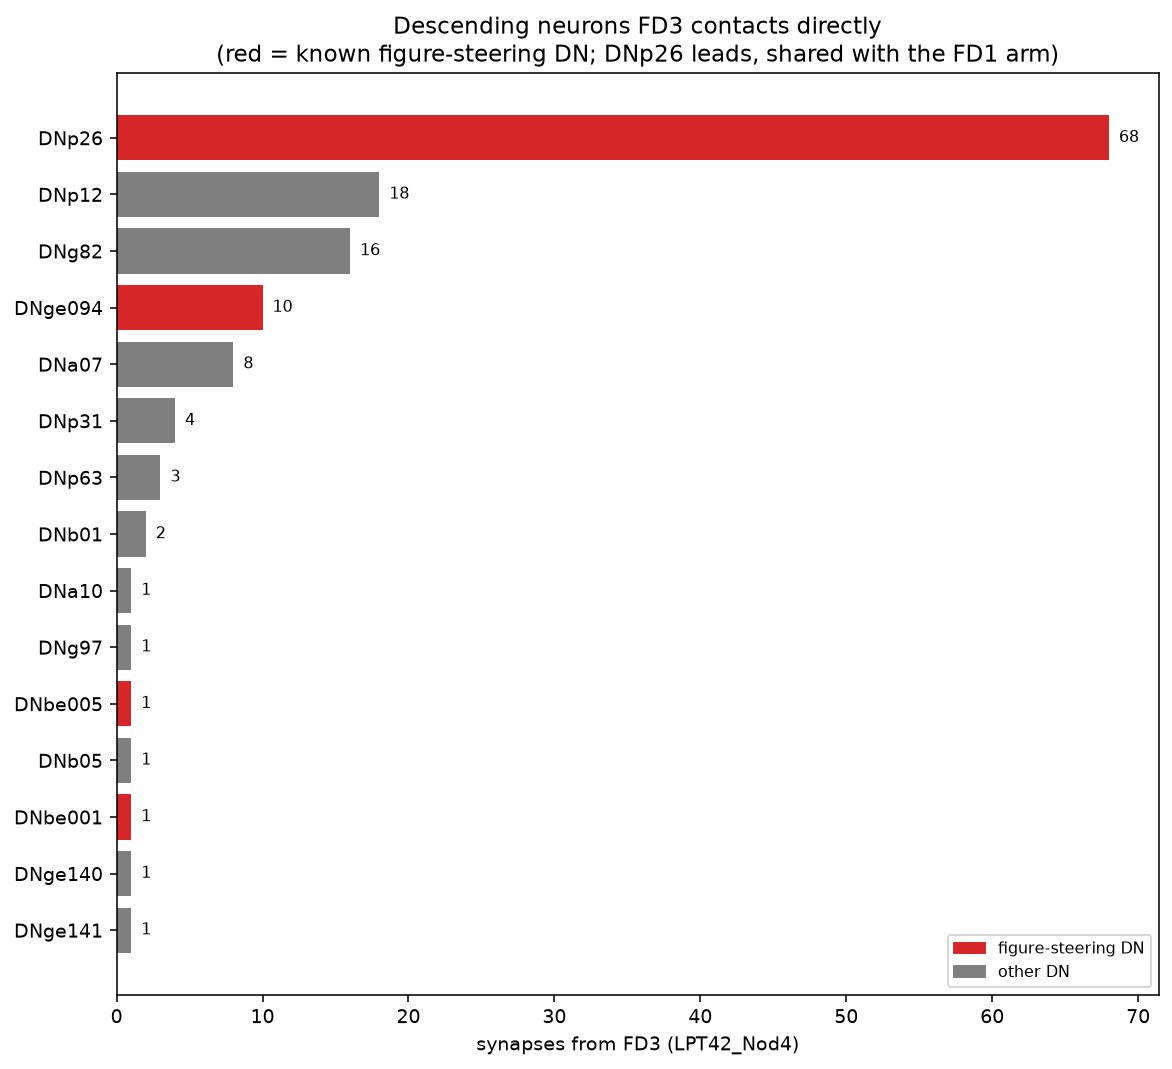
\includegraphics[width=\textwidth]{figures/fd3_dn_ranking.png}
\caption{\textbf{The descending neurons FD3 contacts directly.} Each bar is one descending-neuron type, ranked by the number of synapses it receives from FD3. Red marks neurons already known to drive wing-steering muscles. \ttt{DNp26}, the figure-steering command neuron shared with the FD1 arm, leads.}\label{fig:dnrank}
\end{figure}


\section{The descending neurons FD3 reaches through a relay}

Beyond the neurons it drives directly, FD3 sends most of its output to central brain neurons rather than to descending neurons. Taking FD3's strongest such partners (those receiving at least 30 synapses from FD3 -- 28 cell types, led by \ttt{PLP230}, \ttt{WED075}, \ttt{PLP178}, \ttt{PLP012}, \ttt{LAL203}, \ttt{PLP078}) and following \emph{their} output reaches a further 402 descending neurons (Fig.~\ref{fig:dnchannels}). This relayed route is broad where the direct route is focused: it spreads onto many more descending neurons, the larger of the two routes by total synapses.

Crucially the two routes are not unrelated. 21 descending-neuron types are reached \emph{both} directly and through the relay, including \ttt{DNa10}, \ttt{DNb01}, \ttt{DNb05}, \ttt{DNbe001}, \ttt{DNbe005}, \ttt{DNg34}, \ttt{DNg82}, \ttt{DNg97} -- the figure-steering neurons recur on both paths, so the relay reinforces the same steering output the direct route addresses rather than diverting it elsewhere. Because the size of the relayed set depends on how strong a partner has to be to count, we report that sensitivity explicitly (Fig.~\ref{fig:dnchannels}b): the count grows smoothly as the threshold is relaxed, with no special cut-off doing the work.

\begin{figure}[H]\centering
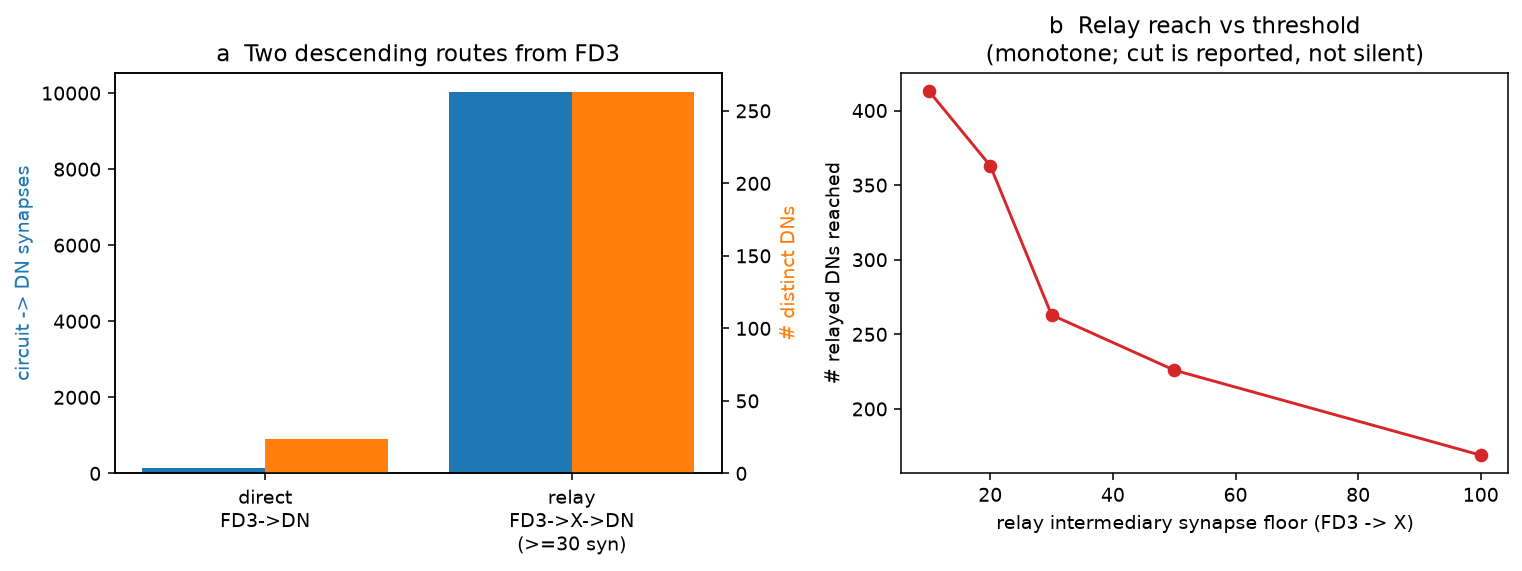
\includegraphics[width=\textwidth]{figures/fd3_descending_channels.png}
\caption{\textbf{Two descending routes from FD3.} (a) The direct route (FD3 $\rightarrow$ descending neuron) is focused; the relayed route (FD3 $\rightarrow$ central partner $\rightarrow$ descending neuron) is broader, reaching many more neurons. (b) The number of relayed descending neurons as the partner-strength threshold is varied -- it changes smoothly, so the result does not hinge on one cut-off.}\label{fig:dnchannels}
\end{figure}


\section{What those neurons command}

Each descending neuron FD3 reaches can be matched, by its standard name, to a cell in the male nerve-cord connectome and from there to the motor neurons and muscles it contacts. Weighting every neuron by how strongly FD3 drives it, the largest share of FD3's descending output -- 42.7\% -- reaches the \emph{wing-steering} muscles (Fig.~\ref{fig:motorsys}), the muscles that adjust the stroke of each wing to turn the fly. Smaller shares reach the neck (gaze), abdominal and haltere systems. The output is thus dominated by the motor system used to steer towards or away from a seen object, exactly the behaviour the FD cells were proposed to serve.

The principal target, \ttt{DNp26}, drives the \emph{contralateral} wing (its wing-steering output goes overwhelmingly to the side opposite its own cell body) through the steering muscles \ttt{hg1}, \ttt{hg2}, \ttt{i1} -- reproducing, from FD3's vantage point, the same muscle targets found on the FD1 arm. A figure seen to one side thus acts, through FD3 and \ttt{DNp26}, on the opposite wing: the asymmetry needed to rotate the body toward (or away from) the object.

\begin{figure}[H]\centering
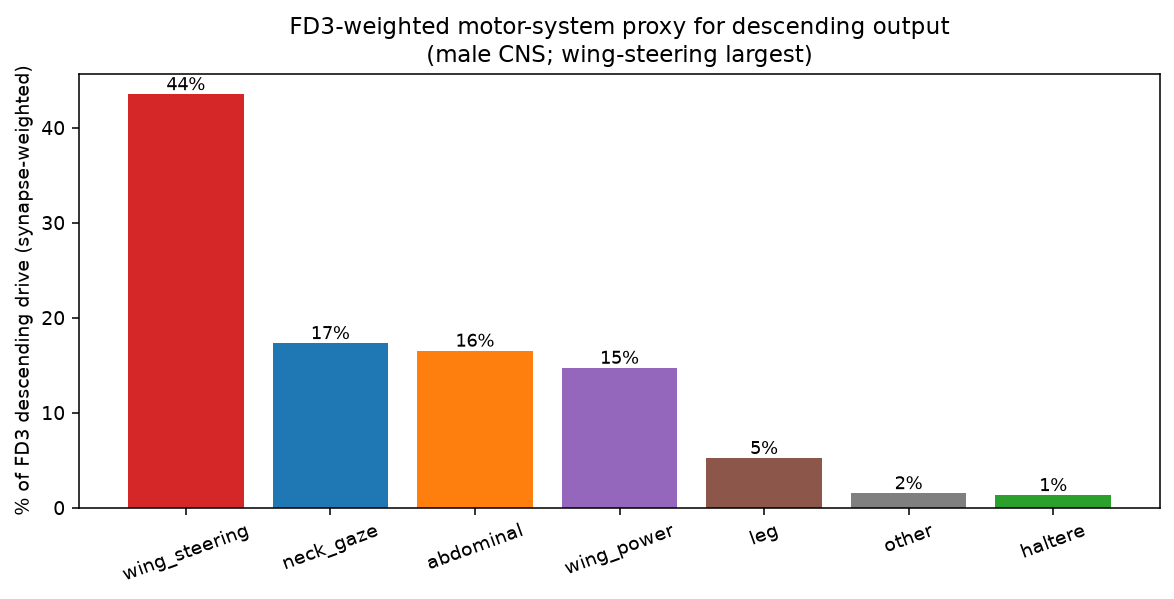
\includegraphics[width=\textwidth]{figures/fd3_motor_systems.png}
\caption{\textbf{What FD3 commands.} The motor systems reached by FD3's descending output, weighted by how strongly FD3 drives each descending neuron. Wing-steering dominates.}\label{fig:motorsys}
\end{figure}


\begin{figure}[H]\centering
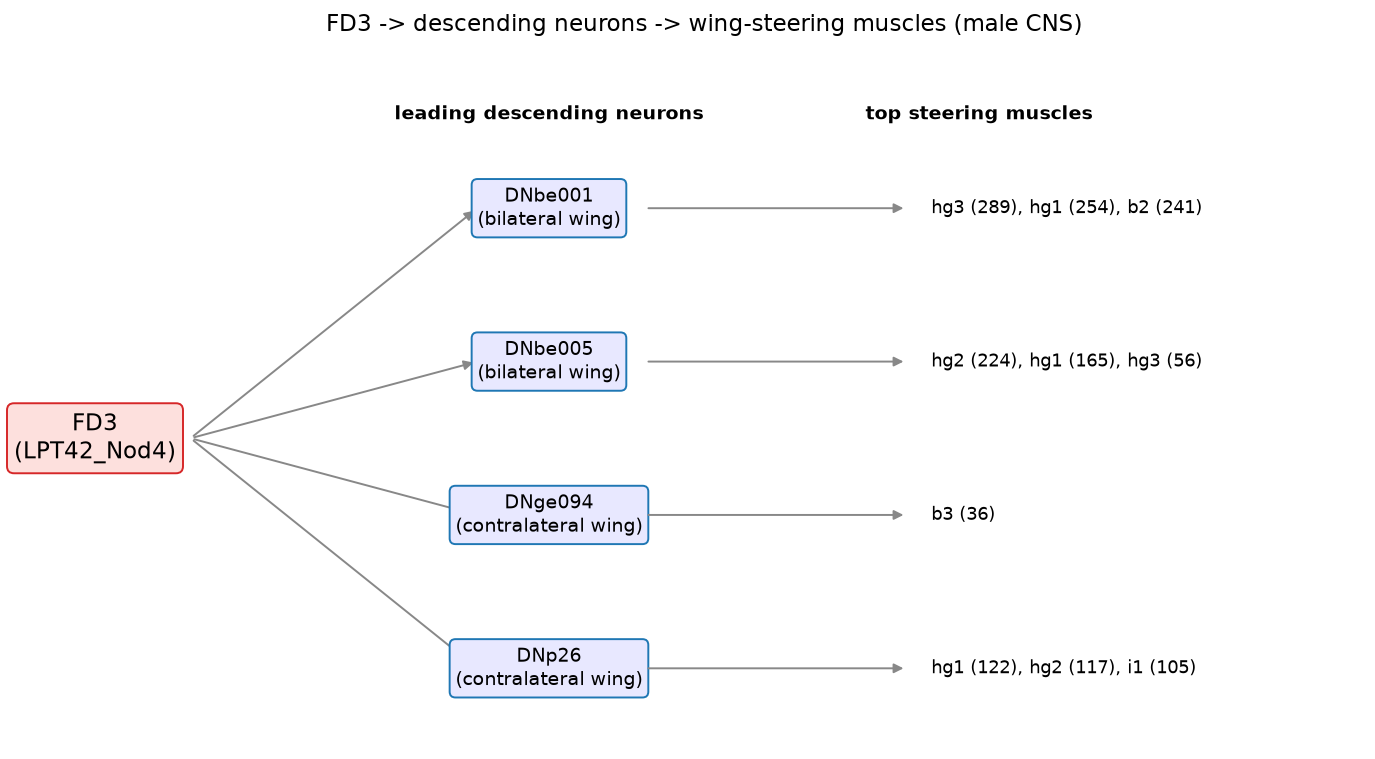
\includegraphics[width=\textwidth]{figures/fd3_brain_to_muscle.png}
\caption{\textbf{From FD3 to the wing muscles.} The leading wing-steering descending neurons FD3 reaches, the wing each one steers, and the steering muscles it drives in the nerve cord.}\label{fig:b2m}
\end{figure}


\section{Functional implications}

Three things follow. First, FD3 is wired as a \emph{steering} cell: its output is directed mainly at the wing-steering muscles, the muscles that turn the fly, rather than at the legs or the escape/jump system. This is the motor counterpart of the behavioural role Egelhaaf proposed for the FD cells -- tracking and fixating a moving figure. Second, FD3 and FD1 converge on the same command neuron, \ttt{DNp26}: the brain appears to pool figure signals of different directions and visual-field positions onto a shared steering output, rather than keeping a separate motor channel per figure cell. Third, the principal pathway is \emph{crossed} -- the dominant steering target acts on the wing opposite the cell body -- which is the correct sign for turning the body in response to an object seen off to one side. Together these place FD3 squarely on the sensory-to-motor arc for figure-directed steering, downstream of the receptive-field properties established in the companion identity report and upstream of the wing muscles.

\section{What the data can and cannot settle}

\textbf{The exact counts depend on the data source.} How many synapses and how many descending neurons FD3 contacts is reported slightly differently by the live and the frozen copies of the connectome -- the live data, which applies no synapse-cleft threshold, lists somewhat more of both -- so the absolute numbers are given as a range that both sources agree on rather than a single figure. Which descending neurons FD3 reaches, and the wing each one steers, do not depend on the source. \textbf{The relay set depends on a threshold.} The direct descending targets are unambiguous -- they are the neurons FD3 synapses onto. The relayed set depends on how strong a central partner must be to be followed; we report the full sensitivity of the count to that choice rather than fixing a single number, and the steering neurons that matter recur across the whole range. \textbf{The muscle map crosses two connectomes.} The muscles each descending neuron drives are read from a second, male nerve-cord connectome, and the link between the two datasets is the shared neuron name. Where a descending neuron carries the same name in both, the match is direct; a neuron without a named nerve-cord counterpart simply contributes no muscle information and is not forced into one. \textbf{FD3 is two cells.} As in the identity report, FD3 is a single left/right pair, so the result rests on the two cells agreeing and on the thousands of synapses each makes, not on a population average.

\section{Methods and provenance}

\textbf{Connectomes.} The descending targets are read from the FlyWire FAFB brain connectome (materialization v783); a neuron counts as descending by its \ttt{super\_class} annotation. The motor read-out is the male whole-CNS connectome (male-cns:v1.0), reached offline; descending neurons are matched between the two by their shared Janelia name. \textbf{Direct route}: postsynaptic partners of \ttt{LPT42\_Nod4} whose super-class is descending, aggregated by type. \textbf{Relayed route}: FD3's strongest non-descending partners (above a reported synapse floor) and their descending output, attributed to the intermediary type, with the count's threshold-sensitivity reported. \textbf{Motor systems}: each descending neuron's male-CNS motor output classified by motor-neuron subclass (wing-steering, wing-power, neck/gaze, haltere, leg, abdominal); wing laterality is the descending neuron's soma side versus the motor neuron's. \textbf{Reproducibility}: regenerated by \ttt{python scripts/paper\_verify.py --only L} and built from the resulting JSON by \ttt{python scripts/fd3\_report.py descending}. Primary track: \ttt{live}.

\begin{thebibliography}{9}
\bibitem{namiki2018} Namiki S., Dickinson M.H., Wong A.M., Korff W., Card G.M. (2018) The functional organization of descending sensory-motor pathways in \textit{Drosophila}. \textit{eLife} 7:e34272.
\bibitem{figground} \textit{Finding a Vision-Behaviour Circuit through Connectomics} (Figure-Ground Circuit study): the VCH $\to$ T4/T5 $\to$ LLPC1 $\to$ Nod1 $\to$ DNp26 $\to$ wing-steering pathway; Tables S10--S15.
\bibitem{dorkenwald2024} Dorkenwald S. et al. (2024) Neuronal wiring diagram of an adult brain. \textit{Nature} 634:124--138.
\bibitem{egelhaaf1985c} Egelhaaf M. (1985) On the neuronal basis of figure-ground discrimination by relative motion in the visual system of the fly. III. Possible input circuitries and behavioural significance of the FD-cells. \textit{Biol. Cybern.} 52:267--280.
\end{thebibliography}

\end{document}